%************************************************
\chapter{User Study}\label{ch:userStudy}
%************************************************

% Intro text, explain why user study, explain experiment form, etc

% Introduce scenarios and tasks. maybe both in tables. 

% include experiment assets such as route images or book chapter.

% mention questionnaire

% data evaluation

% meta values, like age and gender.

% plot priority data

% plot 0-10 scale data

The purpose of the music player described in chapter \ref{ch:implementation} is to examine user behaviour regarding the focused-casual continuum. The idea behind this concept is that users can vary their level of engagement for a certain action while not being bound to interact strictly focused or casual with the device. The three interaction techniques introduced in section \ref{sec:UserInterface} and the variable amount of control they offer to the user create different levels in the focused-casual continuum. \\

\section{Procedure}\label{sec:studyProcedure}
However, the viability and beneficing of the system needs to be confirmed by users in form of a study. Ten participants (2 female, age 21-29 $\overline{x}$=26, $\sigma$=2.47) with different backgrounds were invited. All participants own a smartphone, but only one person owns a smartwatch. Eight participants already had some experience with gesture controlled devices such as the Nintendo Wii or Microsoft's Kinect. Nobody used speech controlled devices beforehand. Every participant was observed while using the music player in six different scenarios that were both private and in public. In each scenario the participants wore the smartwatch on their left wrist and were sometimes more, sometimes less either physically or mentally distracted. Bicycle and headphones were provided but one could bring her own to feel more comfortable. \\

Scenarios and their settings:
\begin{description}
	\item[Office Work]{The participants are seated at a desk in an office. Their task is to copy a text from a sheet of paper to a file on a laptop thus being mentally and physically distracting. This scenario is in a private surrounding.}
	\item[reading on couch]{The participants are seated on a couch in a private living room. Their task is to read a chapter from a book and summarise the content afterwards.}
	\item[Riding a Bicycle]{The participants are riding a bike on a public parking area. Their task is to follow a pre-defined route. The distraction is both mental and physical.}
	\item[joggin]{The participants are jogging the same route as they ride on the bicycle thus being in public and physically distracted.}
	\item[Walking mentally distracted]{The participants are walking a pre-defined public route playing a memory game on a mobile phone. This is mentally distracting. Touch is still possible.}
	\item[Walking physically distracted]{The participants are walking the aforementioned pre-defined public route carrying a bag in their right hand. This is physically distracting.}
\end{description}

To force the participants to interact with the music player, they were tasked with eight coarsely formulated player interactions in each scenario. For every forced interaction the participant could always freely choose between at least two interaction techniques to use, however, scenario constraints made using some techniques more difficult, e.g. using touch on bicycle. The use of each interaction technique was recorded during the experiment session. Table \ref{tab:scenarioTasks} lists the interaction tasks and the possible interaction techniques that generally could have been used.

\begin{table}[h]
	\myfloatalign
	\begin{tabularx}{\textwidth}{XX} \toprule
		\tableheadline{Forced Interaction} & \tableheadline{Possible techniques} \\ 
		\midrule
		1. start a playlist & touch, speech \\
		2. adjust the volume & touch, speech, gesture \\
		3. toggle shuffle & touch, speech \\
		4. \& 6. skip one or more songs & touch, speech, gesture \\
		5. change song relative to a chosen audio feature & touch, speech \\
		6. skip one or more songs & touch, speech, gesture \\
		7. play song from different genre & touch, speech \\
		8. pause current song & touch, speech, gesture \\
		\bottomrule
	\end{tabularx}
	\caption{Interaction tasks for each scenario instructed in this specific order. The skip to next song task was instructed twice in each scenario.}
	\label{tab:scenarioTasks}
\end{table}


\section{Results}\label{sec:studyResults}
In addition to the experiment every participant answered a questionnaire about the experiences they made. First, they were asked to classify their music listening behaviour on a scale from 1 to 5 where 1 means they choose every song they listen to by themselves and 5 means they turn the music on in the morning and turn it off again in the evening. Figure \ref{fig:listenerTypes} shows the distribution of listener types that participated in the experiment. Most people rated themselves to be a mixture of both extreme listening types. This implies that the participants generally interact a lot with a music player.

The answers to the general questions about the experiment (seen in figure \ref{fig:scenarioQuestions}) show an overall agreement on the suitability of the scenarios. 9 out of 10 participants found these or similar scenarios in their everyday life and all participants are regularly listening to music in these situations. Also 9 participants perceived controlling the music player with a smartwatch in contrast to a mobile phone in the scenario contexts as helpful. In General 8 out of 10 participants support the idea of smartwatch aided systems.

\begin{figure}[bth]
	\myfloatalign
	\label{fig:listenerTypes}
	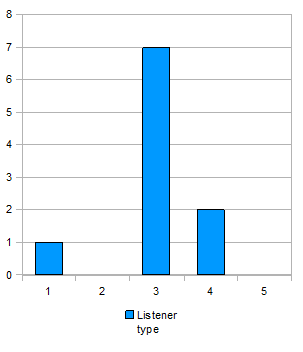
\includegraphics[width=.5\linewidth]{img/listenerTypesPlot.png}
	\caption{Distribution of music listener types. \newline 1 = I choose every song; \newline 5 = I don't care about which song plays.}
\end{figure}

\begin{figure}[bth]
	\myfloatalign
	\label{fig:scenarioQuestions}
	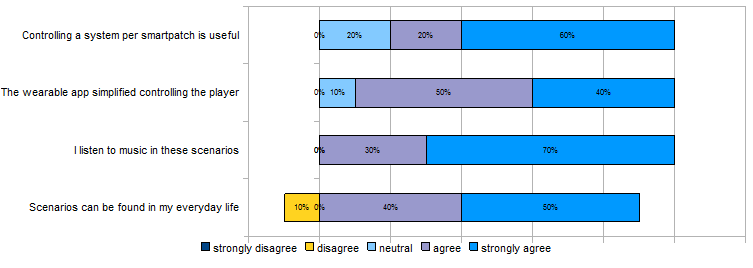
\includegraphics[width=1.2\linewidth]{img/generalQuestionsPlot.png}
	\caption{General questions about the scenarios and smartwatch controlled systems. Answers were made on a five point Likert scale from strongly disagree to strongly agree. Most participants agreed or strongly agreed on all four questions. There were only 3 neutral and 1 disagreeing vote.}
\end{figure}




%Chapter \ref{ch:relatedwork} 


%*****************************************
%*****************************************
%*****************************************
%*****************************************
%*****************************************




